% Substitution matrices
%
% A basic introduction to BLAST substitution matrices

\subsection{Substitution Matrices}
\begin{frame}
  \frametitle{Log-odds Matrices}
  \begin{itemize}
    \item Substitution matrices are a model of evolution, represented by log-odds matrices
    \begin{itemize}
      \item Positive numbers indicate likely substitutions/similarity
      \item Negative numbers indicate unlikely substitutions/dissimilarity
    \end{itemize}
  \end{itemize}
  \begin{center}
   BLOSUM62 \\
   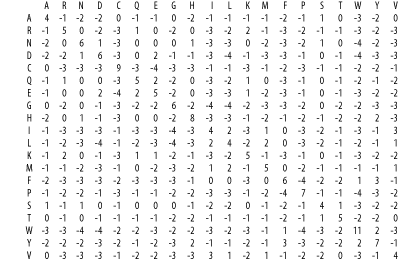
\includegraphics[width=0.5\textwidth]{images/blosum62} 
 \end{center}         
\end{frame} 

\begin{frame}
  \frametitle{Choice of Matrix}
  \begin{itemize}
    \item Substitution matrix determines the raw alignment score $S$
    \begin{itemize}
      \item $S$ is the sum of pairwise scores in an alignment
    \end{itemize}
    \item For proteins:
    \begin{itemize}
      \item \texttt{BLOSUM45 BLOSUM50 BLOSUM62 BLOSUM80 BLOSUM90}
      \item \texttt{PAM30 PAM70 PAM250}
    \end{itemize}
    \item BLOSUM matrices empirically defined from multiple sequence alignments of $\geq n\%$ identity, for \texttt{BLOSUMn}
    \item For nucleotides: `matrix' defined by match/mismatch (reward/penalty) parameters
  \end{itemize}
\end{frame} 
